\subsection{$\llh$ Event Selection}
The $\llh$ channel is the composite of two sub-channels of $\eeh$ and $\mmh$ process. The dominant backgrounds are semi-leptonic $ZZ$ process and other $ZH$ production followed by other types of higgs decay(mainly by higgs decay to off-shell $W$ or $Z$ pair, and both intermediate boson undergo hadronic decay).
Two isolated tracks with opposite charge, reconstructed as electrons or muons, are required in addition to a pair of jets.  The recoil mass provide a very clear signature of the signal events, which have been delicately studied in \cite{CEPC:recoilmass}. 
The cut criteria of lepton pair recoil mass, together with the invariant mass of jet pair and lepton pair, are opptimized to maximum the signal significance. 
The polar angluar of the lepton pair recoil system are more concentrated in central region than the irreducible backgrounds from $t-$channel $ZZ$ production. The distribution of recoil and invariant masses and lepton pair
polar angluar distribution are presented in figure \ref{fig:kinematic_mumuh} and 
\ref{fig:kinematic_eeh} for $\mumuh$ and $\eeh$ analysis.
To reject the background events from other higgs decay, y-value cut was set to suppress events with jet multiplicity other than 2. The signal and dominant backgrounds events yields after applying cuts are summarized in table \ref{tab:mumuh_cut} and \ref{tab:eeh_cut} for $\mmh$ and $\eeh$ analysis respectively.\par


\begin{figure}[!htpb]
\label{fig:kinematic_mumuh}
\centering
\subfigure[]
{
  \begin{minipage}[b]{0.42\textwidth}
  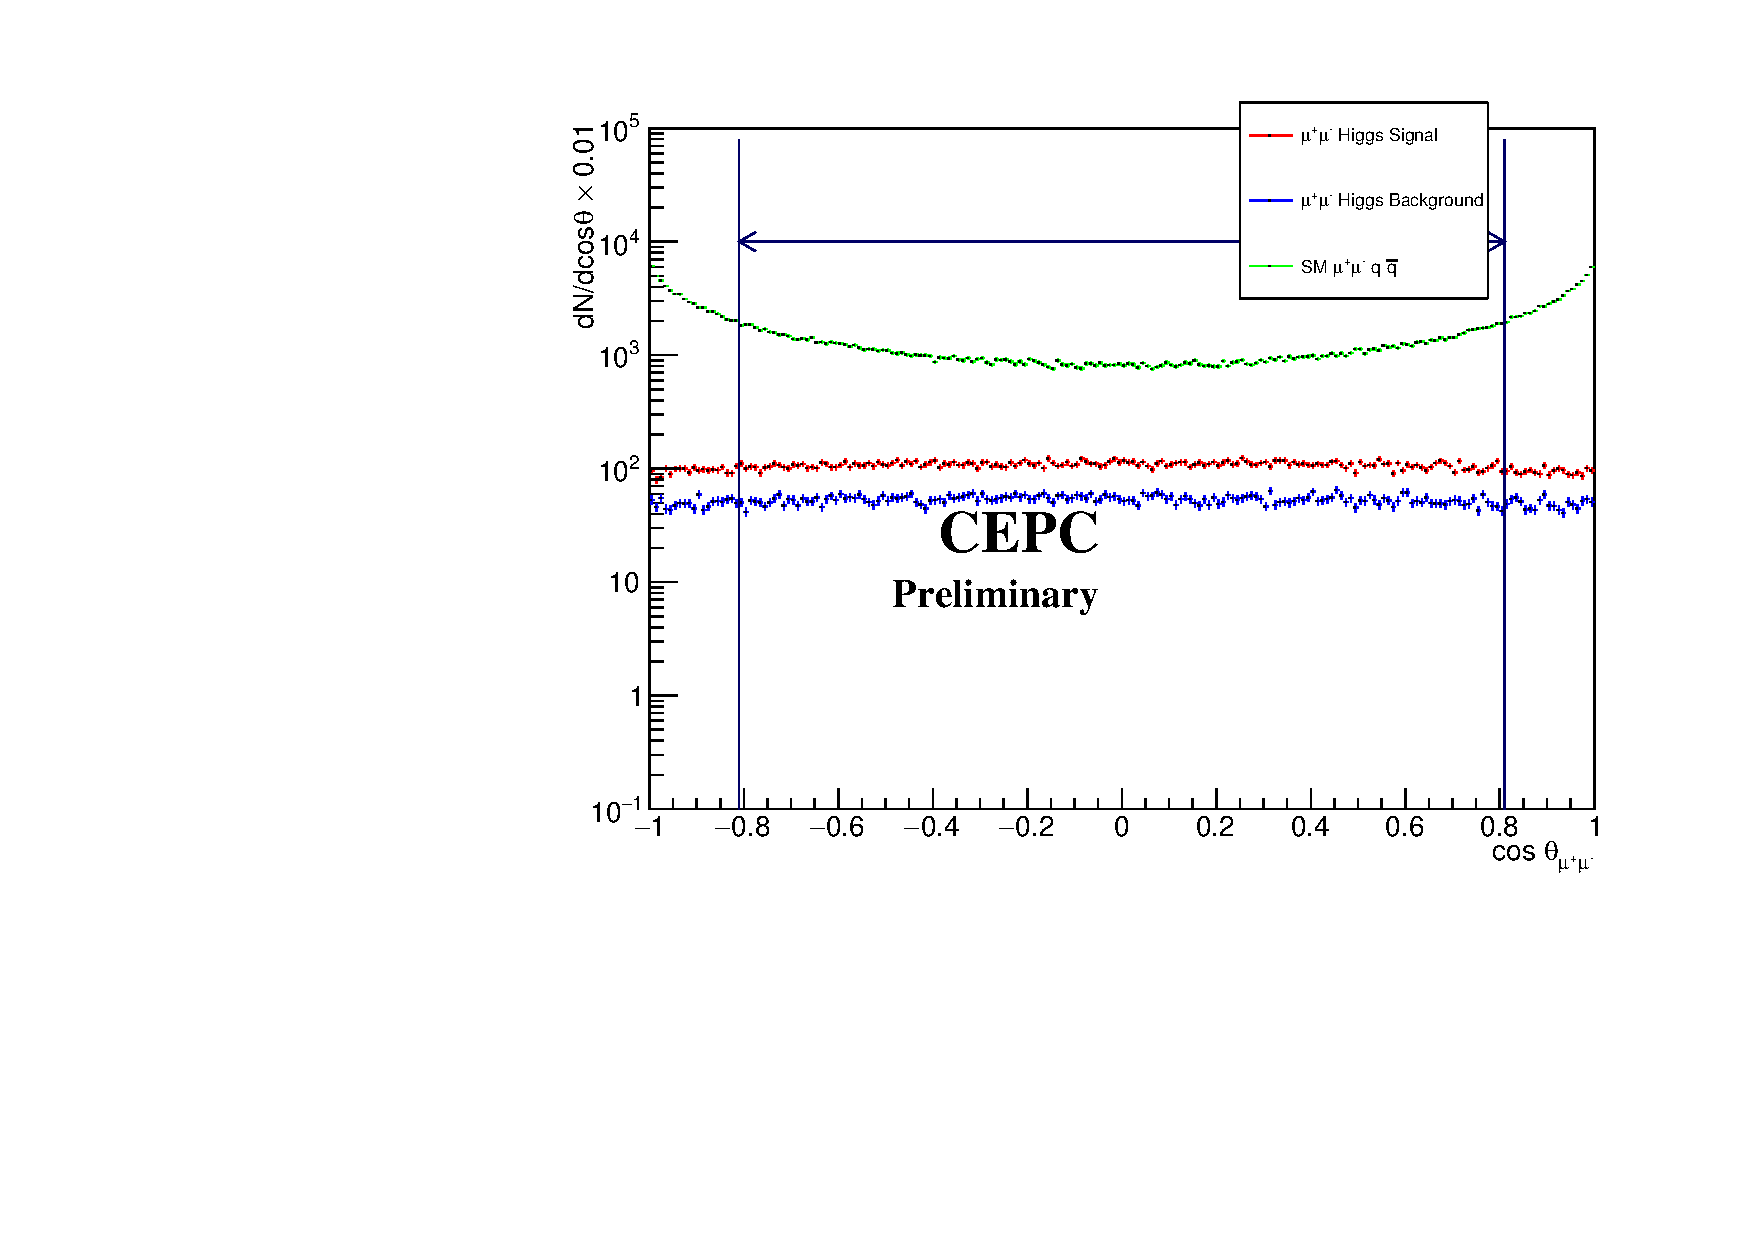
\includegraphics[width=\textwidth]{Analysis/mumuh/ZAngle.pdf}
  \end{minipage}
}
\subfigure[]
{
  \begin{minipage}[b]{0.42\textwidth}
  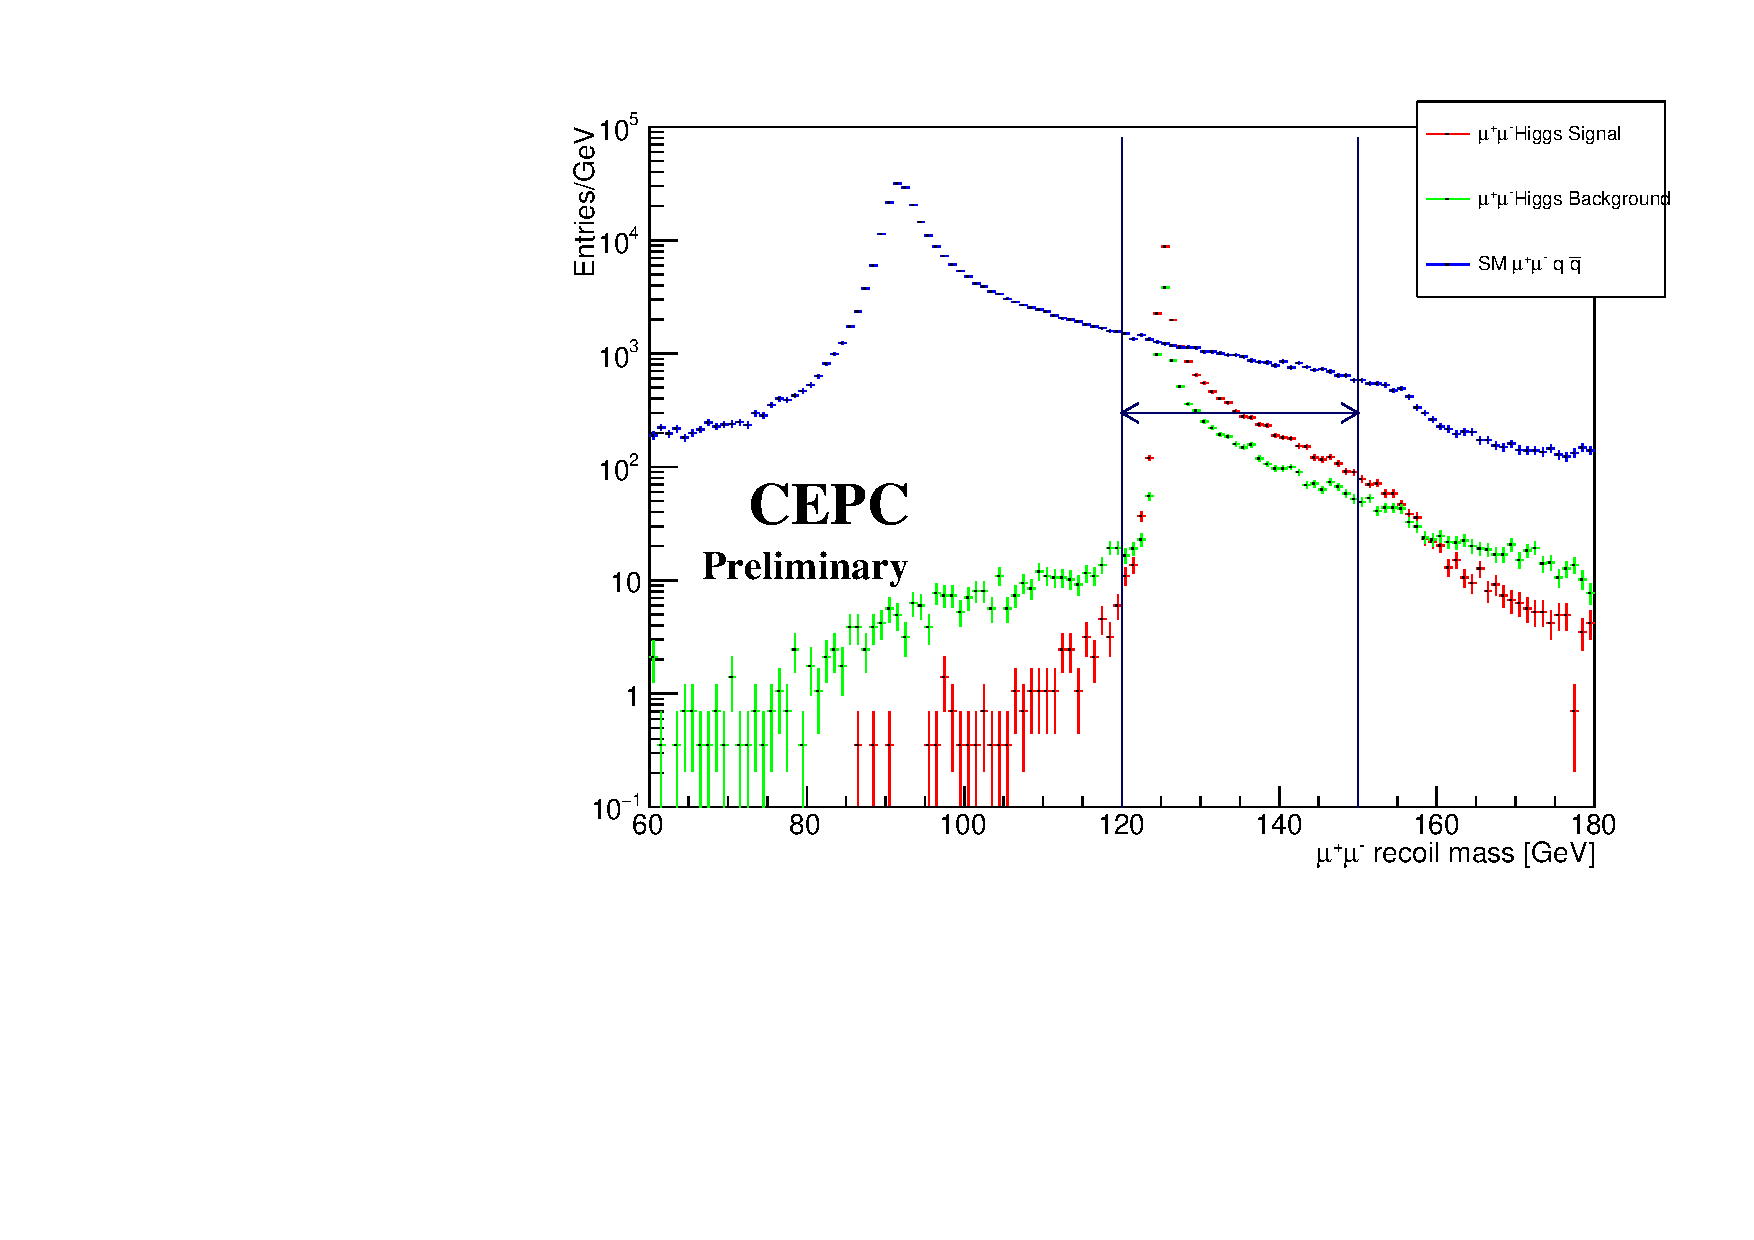
\includegraphics[width=\textwidth]{Analysis/mumuh/mumu_recoil.pdf}
  \end{minipage}
}
\subfigure[]
{ 
   \begin{minipage}[b]{0.42\textwidth}
   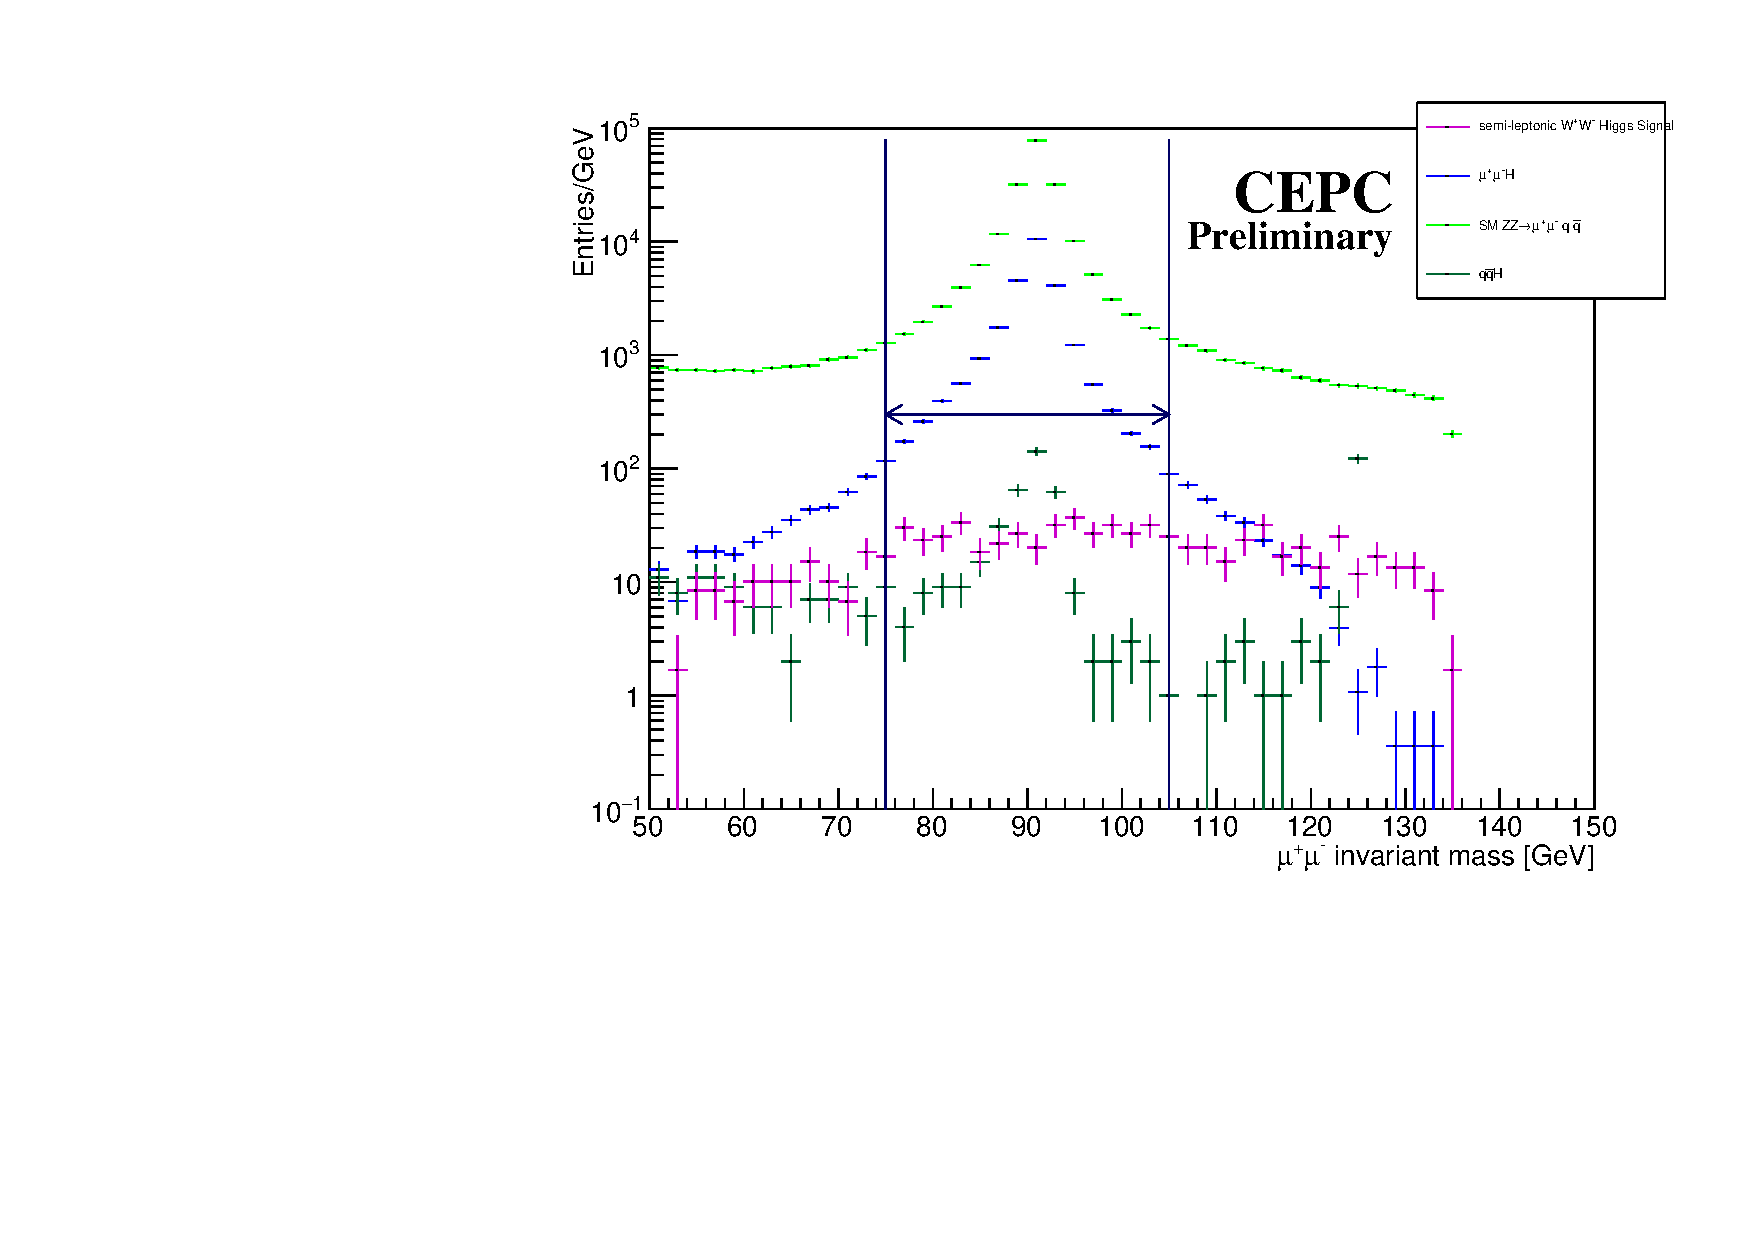
\includegraphics[width=\textwidth]{Analysis/mumuh/mumu_inv.pdf}
   \end{minipage}
}
\subfigure[]
{
    \begin{minipage}[b]{0.42\textwidth}
    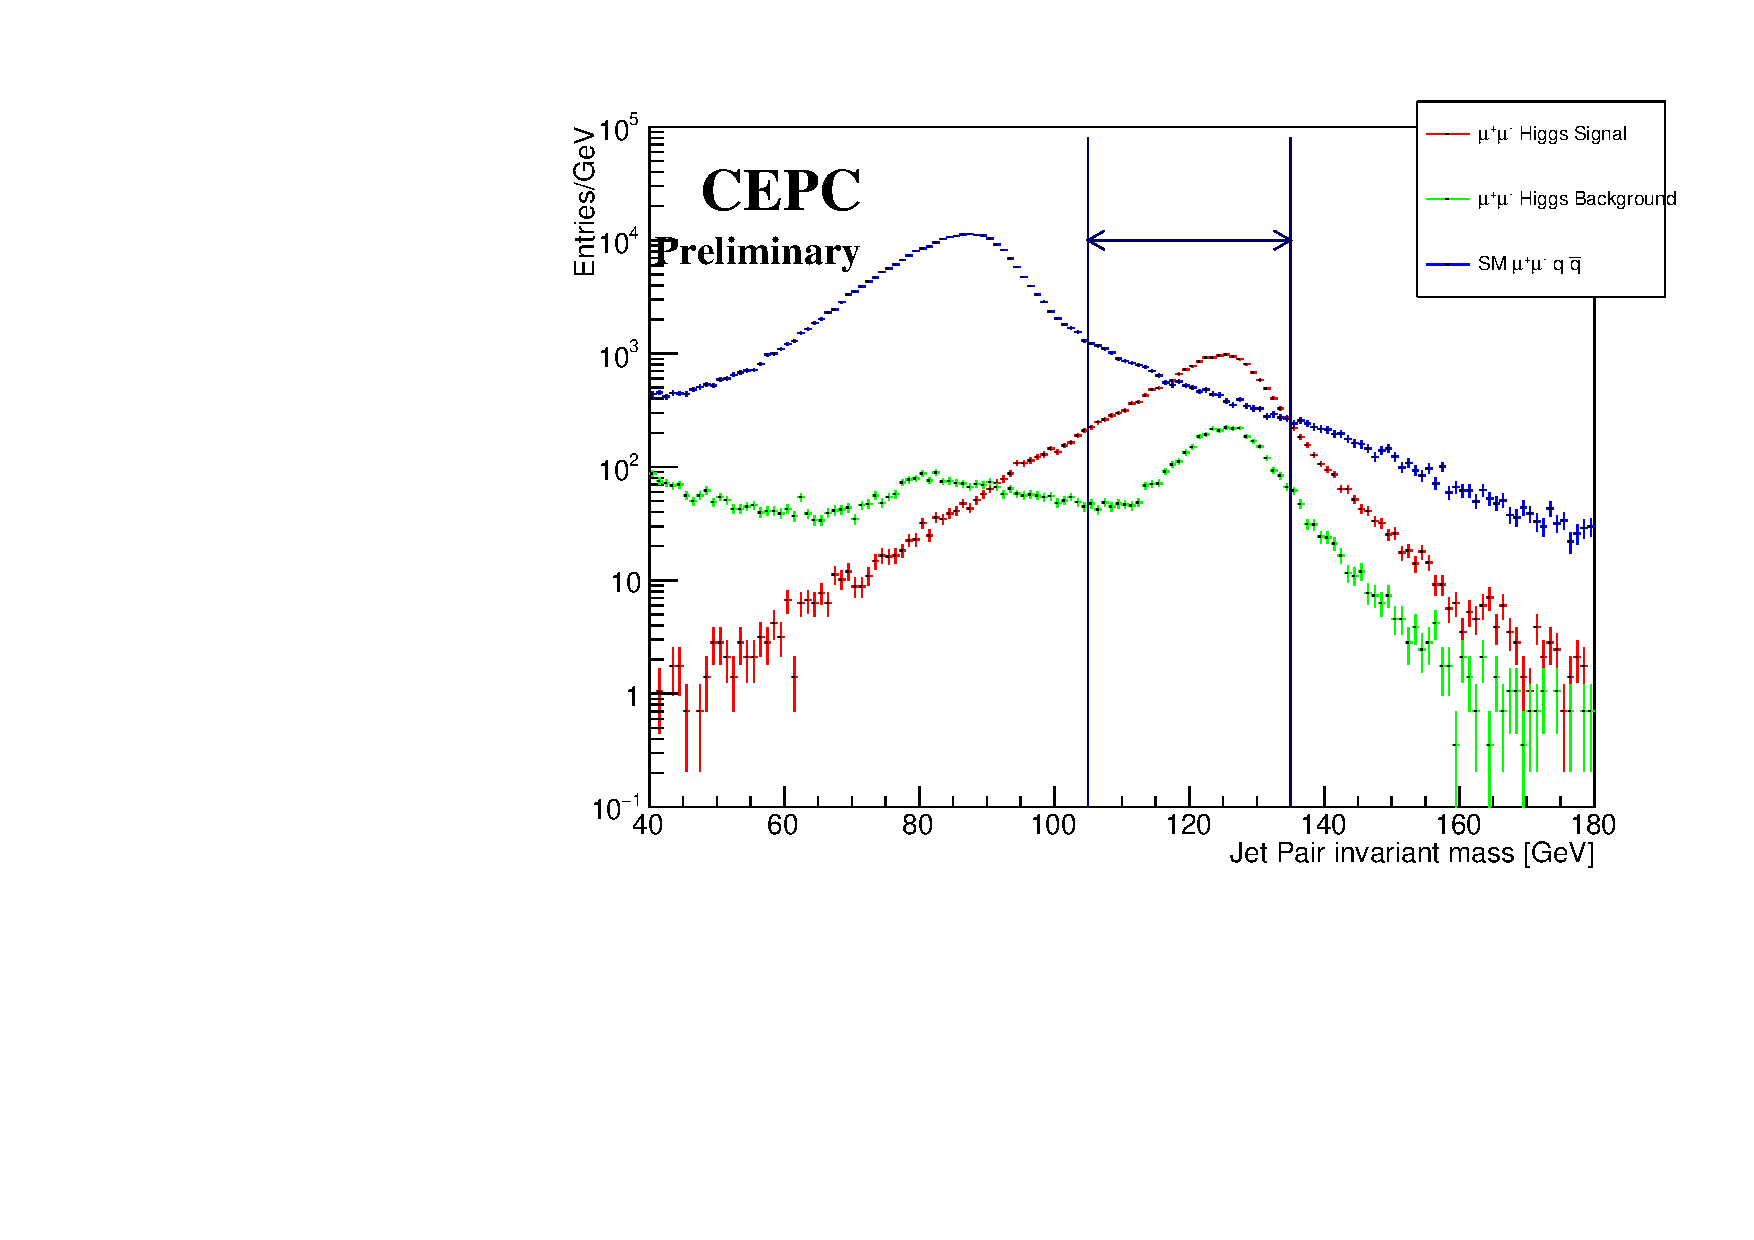
\includegraphics[width=\textwidth]{Analysis/mumuh/JJ_inv.pdf}
    \end{minipage}
}
\caption{Distribution of $\mu^+\mu^-$ system polar angle(top left), $\mu^+\mu^-$ recoil mass(top right), $\mu^+\mu^-$ invariant mass(bottom left) and jet pair invariant mass(bottom right) for signal and dominant backgrounds in $\mmh$ analysis.}
\end{figure}

\begin{table}[!htbp]
\label{tab:mumuh_cut}
\center
\begin{tabular}{c|c|c|c}\hline
%\multicolumn{4}{c|}{$\mmh$} \\ \hline
     Event Yields                          &     Signal   & $\mmh$ background  &  SM $\mu^+\mu^-q\bar{q}$ process \\ \hline
     $\sigma\times$Lumi                    &     24532.3  &      10967.6    &     1051700\\ \hline
       Object Selection                    &     17563.7  &      9203.5                     &    296779.5        \\ \hline
0.85$<\cos\theta_{\mu^+\mu^-}<$0.85        &     18580.8 &      8213.7                         &    193043.4
\\ \hline
120 \GeV$<M_{\mu^+\mu^-recoil}<$150 \GeV   &     17953.2  &      7849.6                       &     19711.2 
\\ \hline 
70 \GeV$<M_{\mu^+\mu^-}<$105               &     17557.1  &      7255.4
&17485.2  \\ \hline
105 \GeV$<M_{JJ}<$135 \GeV                 &     14392.6  &      2927.0 
& 5769.2   \\ \hline
$y_{23}$ \& $y_{34}$ cut                   &     13707.8  &      1575.2 
& 5152.8   \\ \hline 
\end{tabular}
\caption{Event Yields of signal and dominant backgrounds with cuts of $\mmh$ channel, normalized to 5000 \ifb.}
\end{table}

\begin{figure}[!htbp]
\label{fig:kinematic_eeh}
\centering
\subfigure[]
{
  \begin{minipage}[b]{0.42\textwidth}
  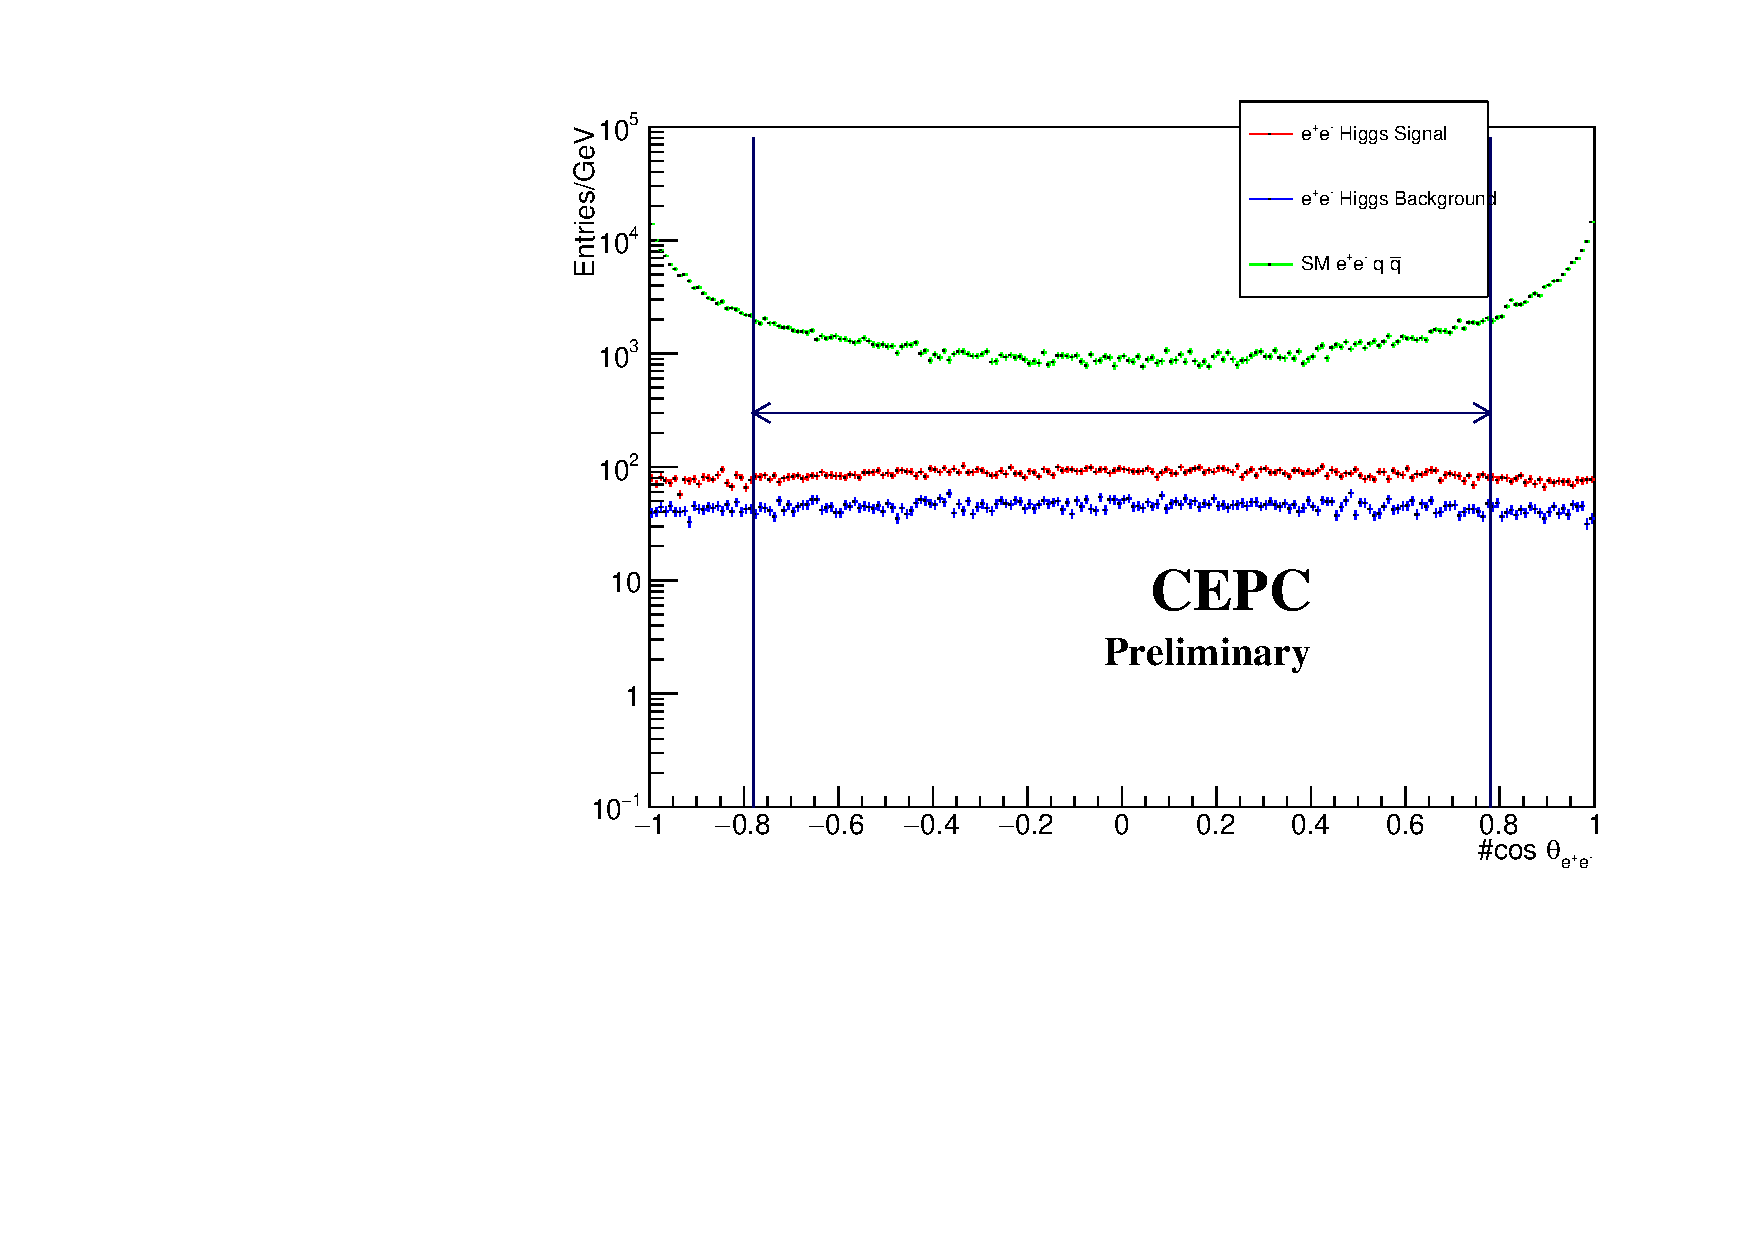
\includegraphics[width=\textwidth]{Analysis/eeh/ZAngle_ee.pdf}
  \end{minipage}
}
\subfigure[]
{
  \begin{minipage}[b]{0.42\textwidth}
  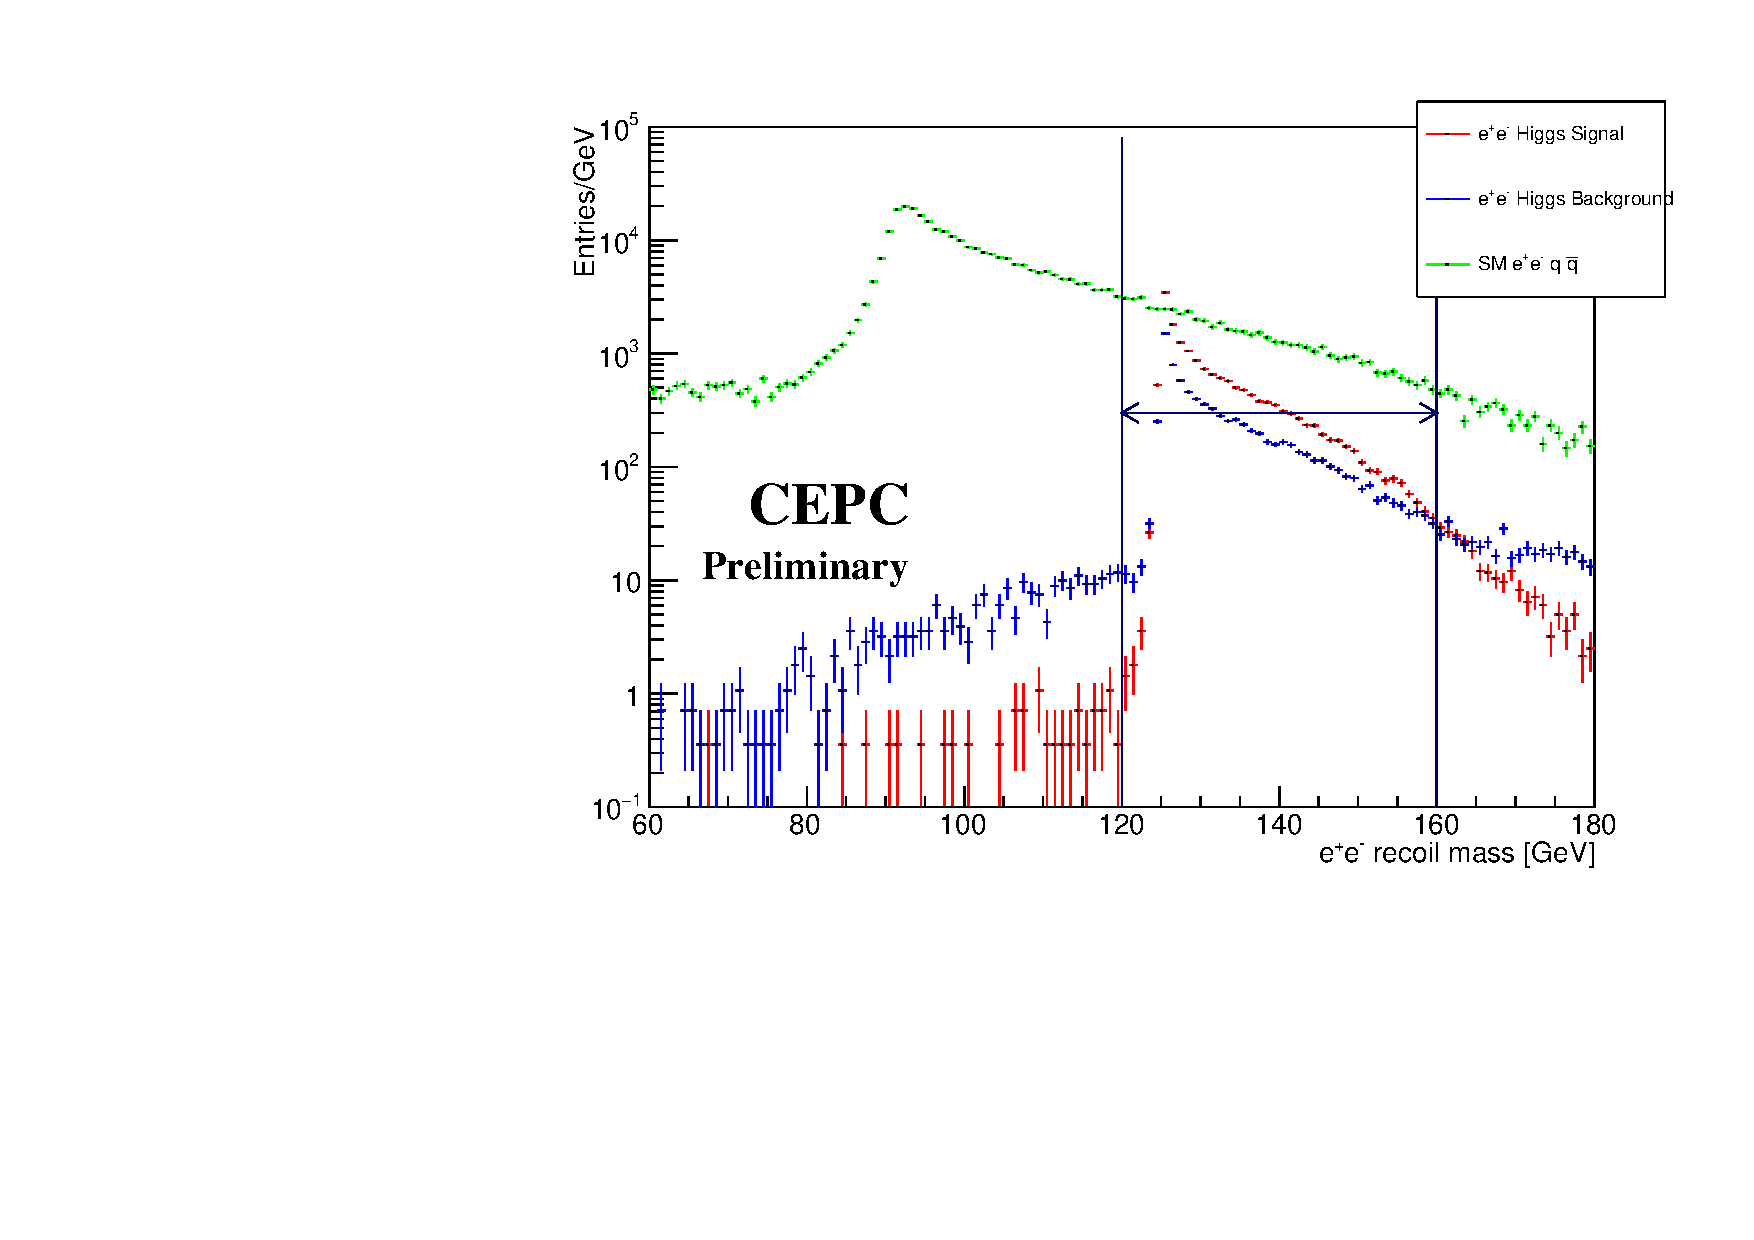
\includegraphics[width=\textwidth]{Analysis/eeh/ee_recoil.pdf}
  \end{minipage}
}
\subfigure[]
{ 
   \begin{minipage}[b]{0.42\textwidth}
   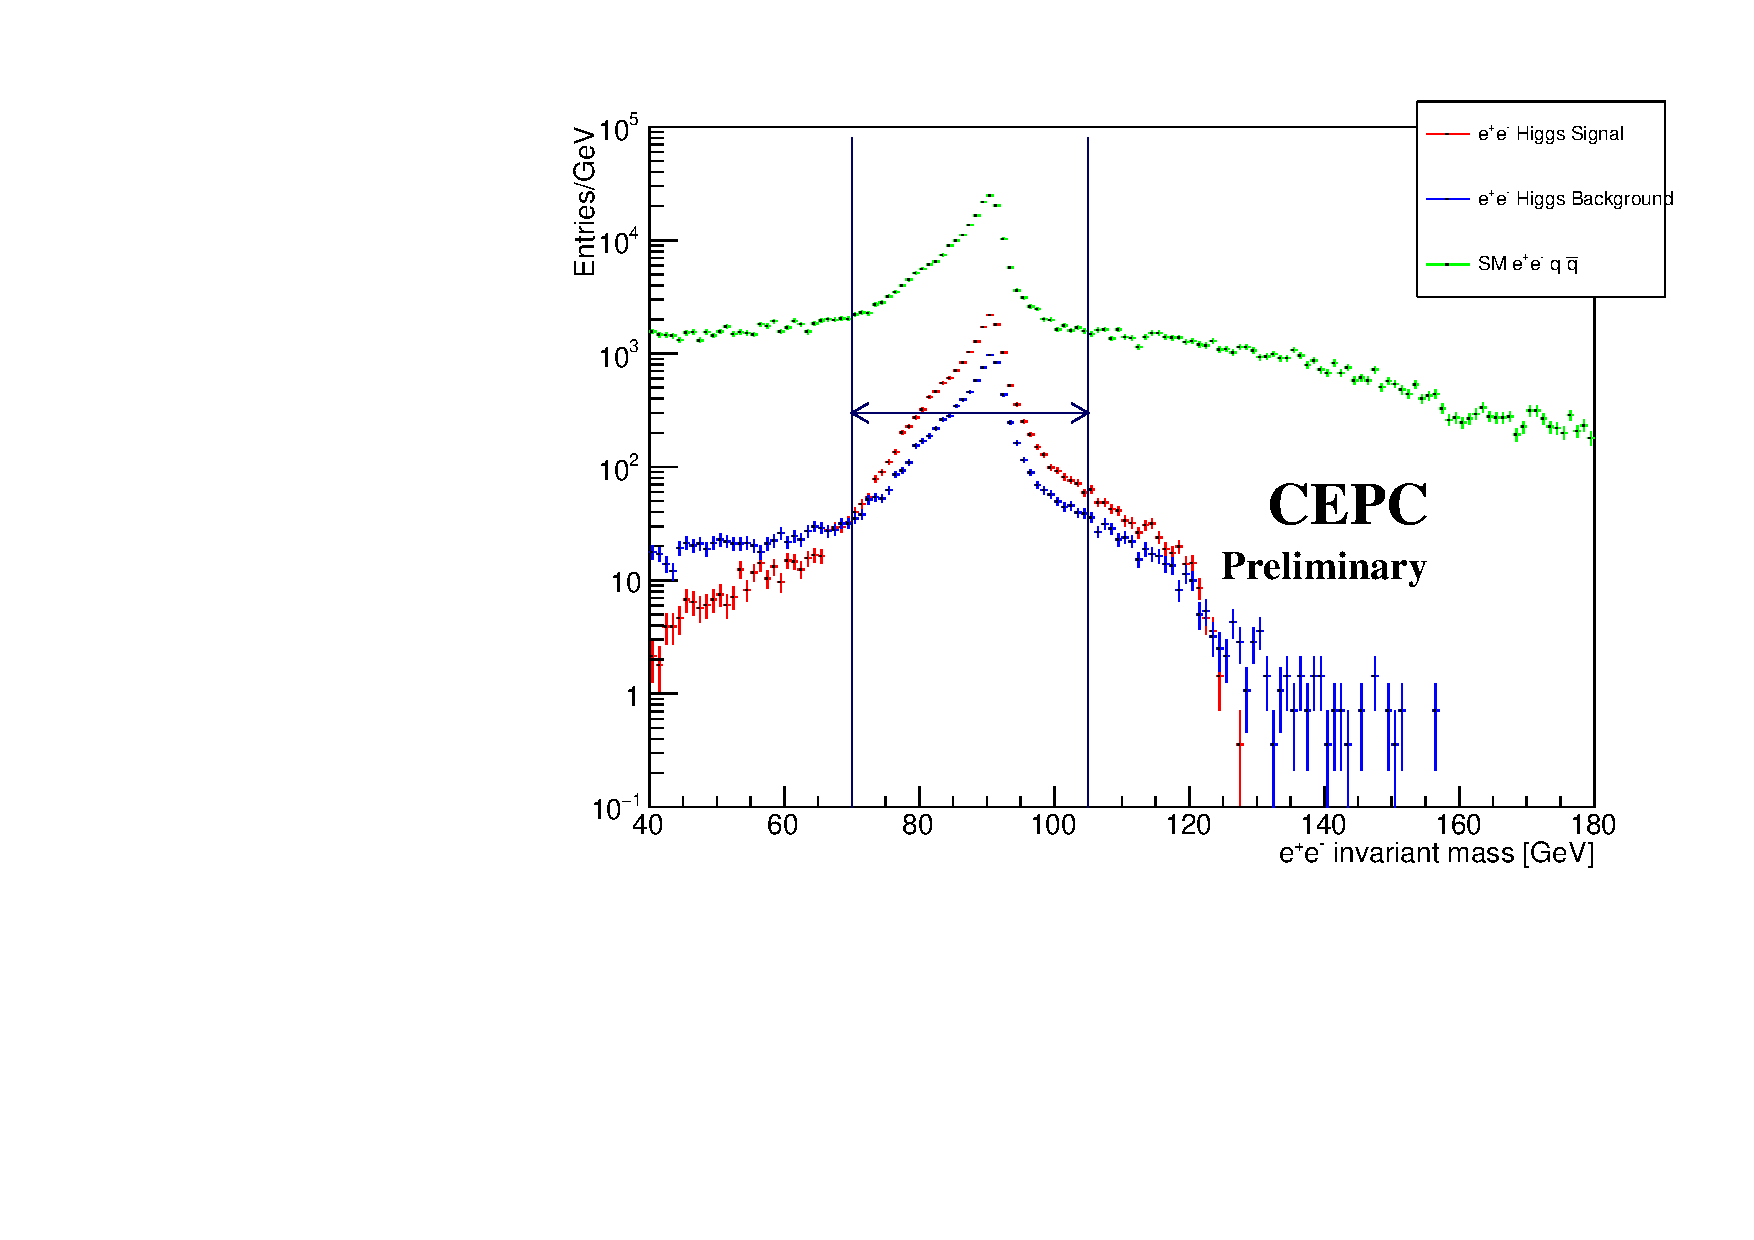
\includegraphics[width=\textwidth]{Analysis/eeh/ee_inv.pdf}
   \end{minipage}
}
\subfigure[]
{
    \begin{minipage}[b]{0.42\textwidth}
    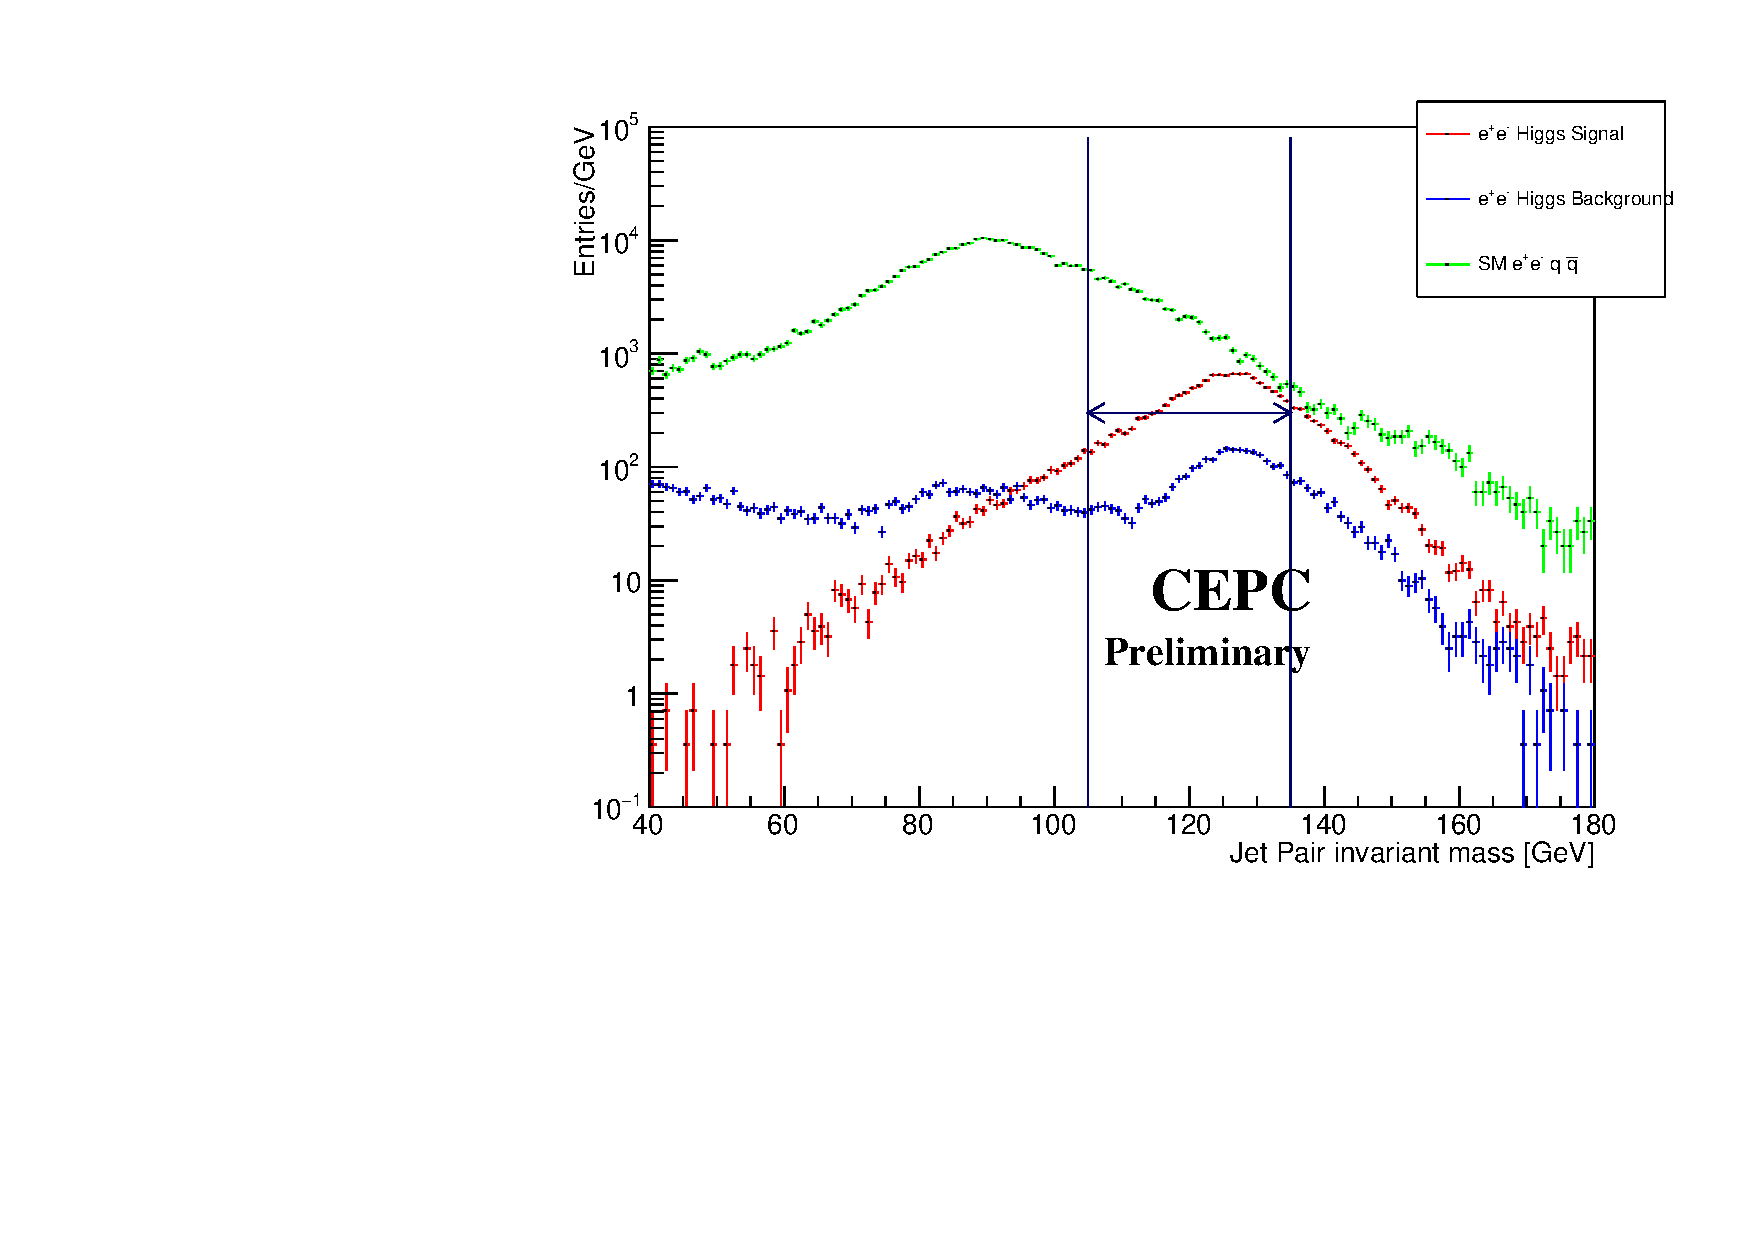
\includegraphics[width=\textwidth]{Analysis/eeh/jj_inv_ee.pdf}
    \end{minipage}
}
\caption{Distribution of $e^+e^-$ system polar angle(top left), $e^+e^-$ recoil mass(top right), $e^+e^-$ invariant mass(bottom left) and jet pair invariant mass(bottom right) for signal and dominant backgrounds in $\eeh$ analysis.}
\end{figure}

\begin{table}[!htbp]
\label{tab:eeh_cut}
\center
\begin{tabular}{c|c|c|c}\hline
%\multicolumn{4}{c|}{$\mmh$} \\ \hline
     Event Yields                          &     Signal   & $\eeh$ background  &  SM $e^+e^-q\bar{q}$ process \\ \hline
     $\sigma\times$Lumi                    &     26438.4  &     11918.6 &   1639129  \\ \hline
       Object Selection                    &     21245.7  &      9192.0                     &    296779.5        \\ \hline
0.78$<\cos\theta_{e^+e^-}<$0.78        &     14002.0  &      7200.8                         &    372942.9
\\ \hline
120 \GeV$<M_{e^+e^-recoil}<$160 \GeV   &     13773.9  &      6581.0                         &    167607.0 
\\ \hline 
70 \GeV$<M_{e^+e^-}<$105               &     13143.0  &      6051.4
&27027.4  \\ \hline
105 \GeV$<M_{JJ}<$135 \GeV                 &     9637.7   &      1935.3 
& 6941.2   \\ \hline
$y_{23}$ \& $y_{34}$ cut                    &    9148.4  &       1101.9 
& 6081.4   \\ \hline 
\end{tabular}
\caption{Event Yields of signal and dominant backgrounds with cuts of $\eeh$ channel, normalized to 5000 \ifb.}
\end{table}
%\clearpage